%!TEX root = ../main.tex

\cleardoublepage
\thispagestyle{plain}
\chapter{Concept map}

\begin{figure}[H]
	\centering
	\hspace*{-1mm}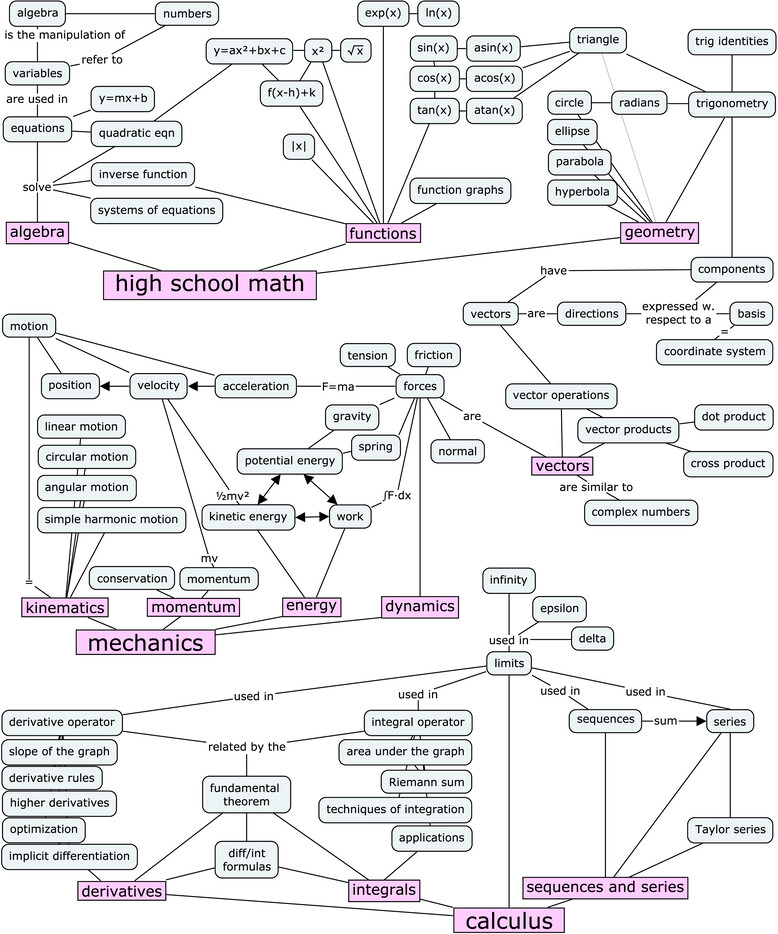
\includegraphics[width=1.06\textwidth]{images/figures/concept_maps/concept_map_full3.jpg}
	\caption{	This diagram shows the connections between the concepts, topics, and subjects covered in the book.
			Seeing the connections between concepts is key to understanding math and physics.\label{fig:big_concept_map}}
	
\end{figure}


\clearpage
\vspace*{5mm}
\noindent
You can annotate the concept map with your current knowledge of each concept to keep track of your progress through the book.
\begin{itemize}
	\item Add a single dot ($\bullet$) next to all concepts you've heard of.
	\item Add two dots ($\bullet\bullet$) next to concepts you think you know.
	\item Add three dots ($\bullet\!\bullet\!\bullet$) next to concepts you've used in exercises and problems.
\end{itemize}
By collecting some dots every week,
you'll be able to move through the material in no time at all.

\bigskip
If you don't want to mark up your book,
you can download a printable version of the concept map here: 
\href{https://bit.ly/mathphyscmap}{\texttt{bit.ly/mathphyscmap}}.


\clearpage
\thispagestyle{plain}

